We have seen in the previous section that speaker identification performance is essentially bi-modal: either a speaker is not recognized at all or it is very well recognized. This section aims at uncovering the speaker characteristics explaining why some speakers are recognized ($\checkmark$) and others are not ($\times$)? To answer this question, we first try to automatically classify the speakers into those two classes. In case we succeed, by analyzing the speaker characteristics contributing the most to this prediction, we should be able to identify the characteristics that facilitate or hamper the identification.

\subsection{$SpkShow$ characteristics}

Numerous characteristics could explain why a $SpkShow$ is recognized or not, including linguistic or prosodic characteristics or the background noise. In this paper, we only study two families of characteristics -- derived from the amount of training data used for speaker modeling, or related to the distribution of speech segments uttered by each speaker in the test set. 

The first set of characteristics includes the duration of training data available for each reference speaker (from the REPERE corpus, other corpora, or both) and the corresponding number of training sessions. For each $SpkShow$, these characteristics are obtained from the oracle system (\emph{i.e.} the system that performs the best for this particular $SpkShow$ among the three systems).

For each $SpkShow$, the second set of characteristics includes the number of speech turns, their total (or average) duration or the duration of the longest speech turn. It also includes characteristics related to the level of interactions of a $SpkShow$, such as the number and total duration of overlapped speech segments or the average pause duration before and after each speech turn of a $SpkShow$.

\subsection{Prediction of oracle performance}

Given a $SpkShow$ and its corresponding set of characteristics, we aim at predicting whether the oracle system is able to (at least partially) recognize $\checkmark$ it or not (at all) $\times$. 
As the corpus is limited (only 305 different $SpkShow$) and unbalanced (63 $\times$ vs. 242 $\checkmark$), we proceed using leave-one-out cross-validation and evaluate this classification experiment as two complementary detection tasks using precision, recall and F-measure.

Not all $SpkShow$ characteristics are meaningful features for this task, and some can even degrade the classification performance. 
Hence, feature selection is applied using the following heuristic manner.
Starting with the whole set of characteristics, each iteration removes the single characteristic whose removal leads to the best performance.
The optimal subset of characteristics is selected as the one leading to the best overall performance.

As far as the classification algorithm is concerned, we chose to use a decision tree (rather than a more sophisticated black box classifier) as the analysis of its internal structure allows for easy interpretation of the results and the importance of each characteristic.
Table~\ref{tableresult} contains the experimental results. It shows that it is possible to predict whether a $SpkShow$ will be recognized ($\checkmark$ $\text{F-measure} = 95.0\%$) or not ($\times$ $\text{F-measure} = 81.4\%$)
\begin{table}[t]
\begin{center}
\begin{tabular}{|r|c|c|c|c|c|c|}
\hline
& \multicolumn{3}{c|}{All characteristics} & \multicolumn{3}{c|}{Optimal subset} \\
\hline
& P. & R. & F-measure & P. & R. & F-measure \\
\hline
$\checkmark$ & 94.5 & 93.4 & 94.0 & 95.6 & 94.6 & 95.0 \\
\hline
$\times$ & 75.8 & 79.0 & 77.4 & 80.0 & 82.7 & 81.4 \\
\hline
\end{tabular}
\caption{Prediction performance}
\label{tableresult}
\end{center}
\end{table}

\subsection{What makes a speaker recognizable?}

Now that we showed that it is possible to predict whether a $SpkShow$ is recognizable or not, this section aims at providing more insight into why this is the case.

Figure~\ref{fig:featureImportance} provides the distributions of \emph{feature importance} for the six characteristics selected in the optimal subset, computed over the 305 leave-one-out cross-validation rotations. 
Here, in the case of decision trees, feature importance is defined as the Gini coefficient and is related to the number of times a characteristic is used in the tree and how discriminant it is on average. More information on this metric can be found in~\cite{Breiman2001}
\begin{figure}[t]
\centering
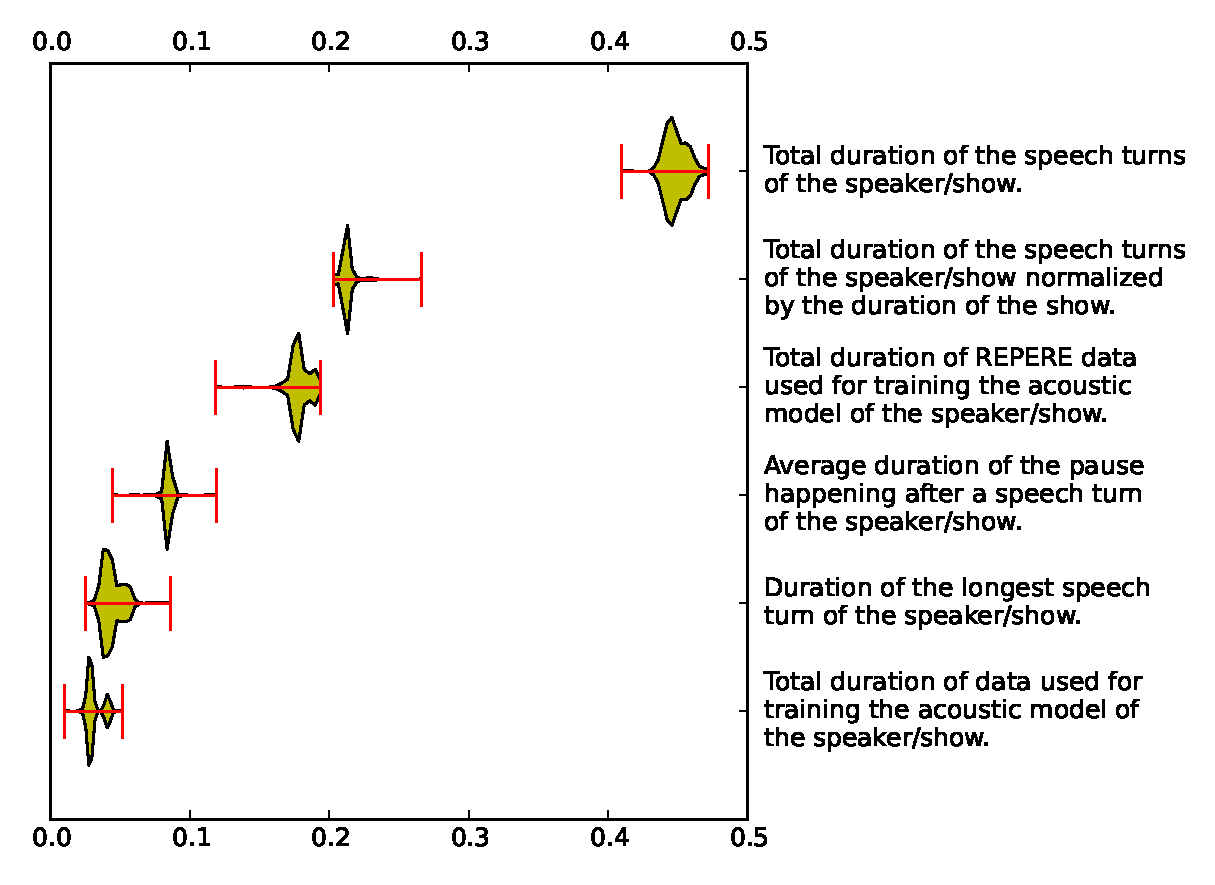
\includegraphics[width=\linewidth]{figures/violin.eps}
\caption{Distribution of feature importance.}
\label{fig:featureImportance}
\end{figure}

Interestingly, the two most important features are related to the duration of speech turns in the test set -- characteristics related to the amount of training data only appear at rank \#3 and \#6. 
The presence at rank \#4 of the characteristic defined as the average duration of the pause after each speech turn of a speaker is somewhat suprising. This could be explained by the fact that long pauses between two speech turns of two different speakers may ease the segmentation process (whose influence is discussed in Section~\ref{sec:analysis}) and therefore increase speaker recognizability.
Finally, Figure~\ref{fig:tree} is a graphical illustration of a decision tree (limited to depth 3) trained on the whole set of $SpkShow$ and based on the optimal subset of characteristics discussed in previous section.
Talkative $SpkShow$ appear to be much easier to recognize than those with only a few short speech turns. When combined with lots of training data (see rightmost leaf), the former characteristic nearly always leads to good recognition (193 $\checkmark$ out of $305$ speakers!).
\begin{figure}[t]
\centering
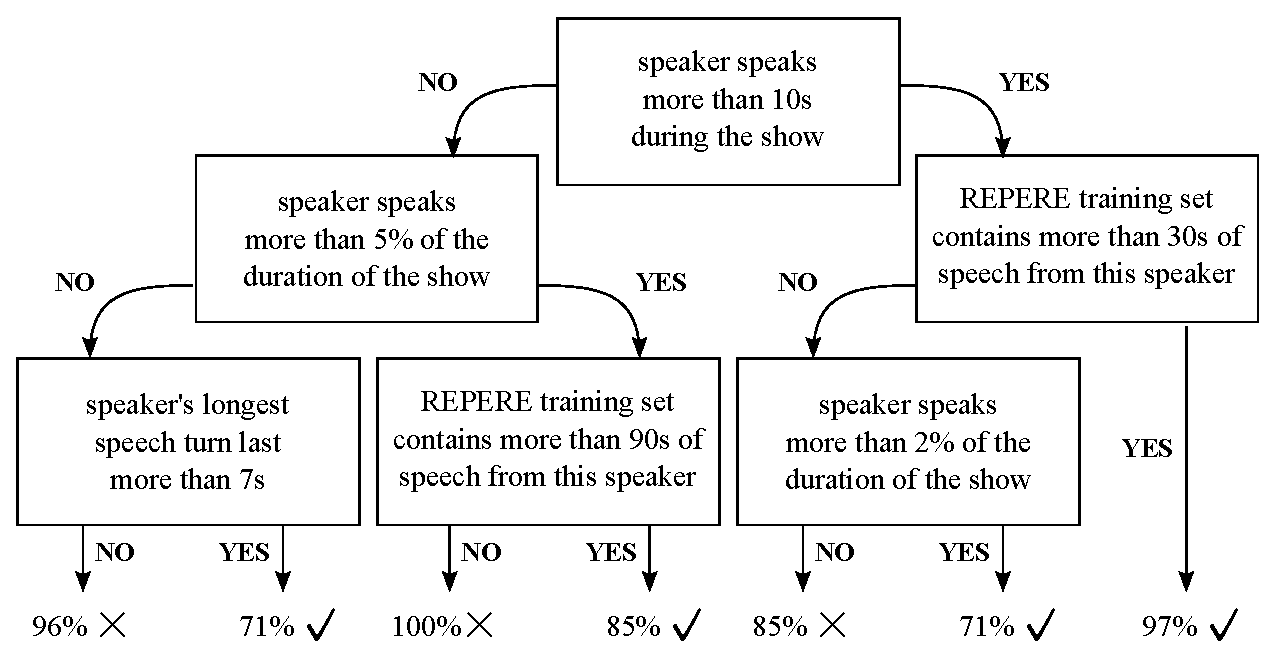
\includegraphics[width=\linewidth]{figures/tree.eps}
\caption{Not recognized ($\times$) vs. (partially) recognized ($\checkmark$)}
\label{fig:tree}
\end{figure}



% As anticipated, the amount of training data appears to be
